\documentclass[11pt]{article}
\usepackage[margin=2.2cm]{geometry}
\usepackage{graphicx, booktabs, hyperref, float, amssymb}
\graphicspath{{../figures/}}
\title{Y-88 Source Scan: Compton-Edge Energy Calibration of the MX17
       Plastic, Liquid, and SiPM-Wall Channels\\
       \large n\_TOF EAR2 X17 campaign, runs 224476--224479 (July 17, 2026)}
\author{Dylan Neff \\[0.5ex] {\small analysis and document prepared with Claude (Anthropic AI assistant)}}
\date{July 18, 2026}

\begin{document}
\maketitle

\begin{abstract}
Four dedicated $\sim$13-minute source runs (224476--79, one per arm A/B/C/D)
were taken the morning of 2026-07-17 with a single $^{88}$Y source placed
between the two plastic scintillator bars of one arm. $^{88}$Y emits 898 and
1836\,keV $\gamma$s; in organic scintillator the observable landmarks are the
Compton edges at \textbf{699} and \textbf{1612\,keVee}. Despite $\sim$30\,s of
effective live time the source is bright ($>$3\,M plastic hits on the
illuminated arm), so the spectra are smooth. The runs were reprocessed
privately with R.~Mucciola's PSA UserInput (WALL + LIQ pulse-shape fitting) so
the liquid scintillators appear in the readout for the first time. Three
results. (1)~\textbf{Both plastic Compton edges are resolved on every
illuminated channel}, fit as two \emph{independent} smeared steps: the measured
1612/699 ratio (median 2.4, per channel 1.8--2.6) reproduces the expected 2.31,
confirming the energy assignment from the data itself; the plastic response is
linear to $\sim$10--20\%. The plastic HV was clearly \textbf{raised} for these
``plastic calibration'' runs --- the 699 edge sits at 20--27\,mV,
$\sim$25--39\,mV/MeVee. (2)~\textbf{First liquid-scintillator absolute energy
scale}: the 699\,keVee Compton edge is a clean bump at 22--26\,mV on all four
liquids (32--37\,mV/MeVee), remarkably consistent arm-to-arm. (3)~The same edge
appears at 20--30\,mV on the source-facing SiPM-wall channels (the new PSA also
suppresses the wall noise hits by $\sim$10$\times$). Across all three detector
types the 699\,keVee edge lands within 21--27\,mV per arm. The exact run HV is
not recorded in the data and is required to transport the plastic scale to
nominal HV.
\end{abstract}

\section{Runs, reprocessing, and method}
The run/arm assignment is 224476$=$A, 224477$=$B, 224478$=$C, 224479$=$D
(source between that arm's plastic bars, near the middle, so both bars, the
arm's wall, and the liquid vessel behind are illuminated). The runs are
beam-off ($\sim$1500 timer triggers, 20\,ms windows), so the beam-analysis
selection is inapplicable: all triggers are used and \texttt{tof}/\texttt{tflash}
are ignored. The official processed files carry no LIQ trees (they predate the
LIQ PSA UserInput), so the four runs were reprocessed with the official
\texttt{RunProcessing.sh} pipeline and Mucciola's
\texttt{UserInput\_2026\_EAR2\_X17.h} (pulse-shape fitting for WALL and LIQ);
this both adds the liquids and cleans the wall reconstruction (WALL noise hits
drop by $\sim$10$\times$ relative to the official files). Hits are extracted
with the existing cache (\texttt{fastread/extract\_hits}), histogrammed in
linear mV (0.2\,mV bins) and converted with the per-run DAQ full-scale factors
($\sim$0.031\,mV/ADC).

Edge extraction works on the \emph{linear} $dN/dA$ spectrum. The two plastic
gammas produce a Compton continuum that steps down at each edge; each edge is
fit \emph{independently} as a single resolution-smeared step (complementary
error function on a background), the 698.63\,keVee edge as the dominant step and
the weaker 1612.06\,keVee edge in the window above it --- so their ratio is a
measured cross-check, not an input. On the SiPM walls and the liquids the
699\,keVee edge instead appears as a localised bump and is fit as a Gaussian on
a linear background, the peak centre being the landmark. All errors are Poisson
bootstraps (200 resamples, fixed seed) of the fine bins, floored at half a bin.

\begin{figure}[H]\centering
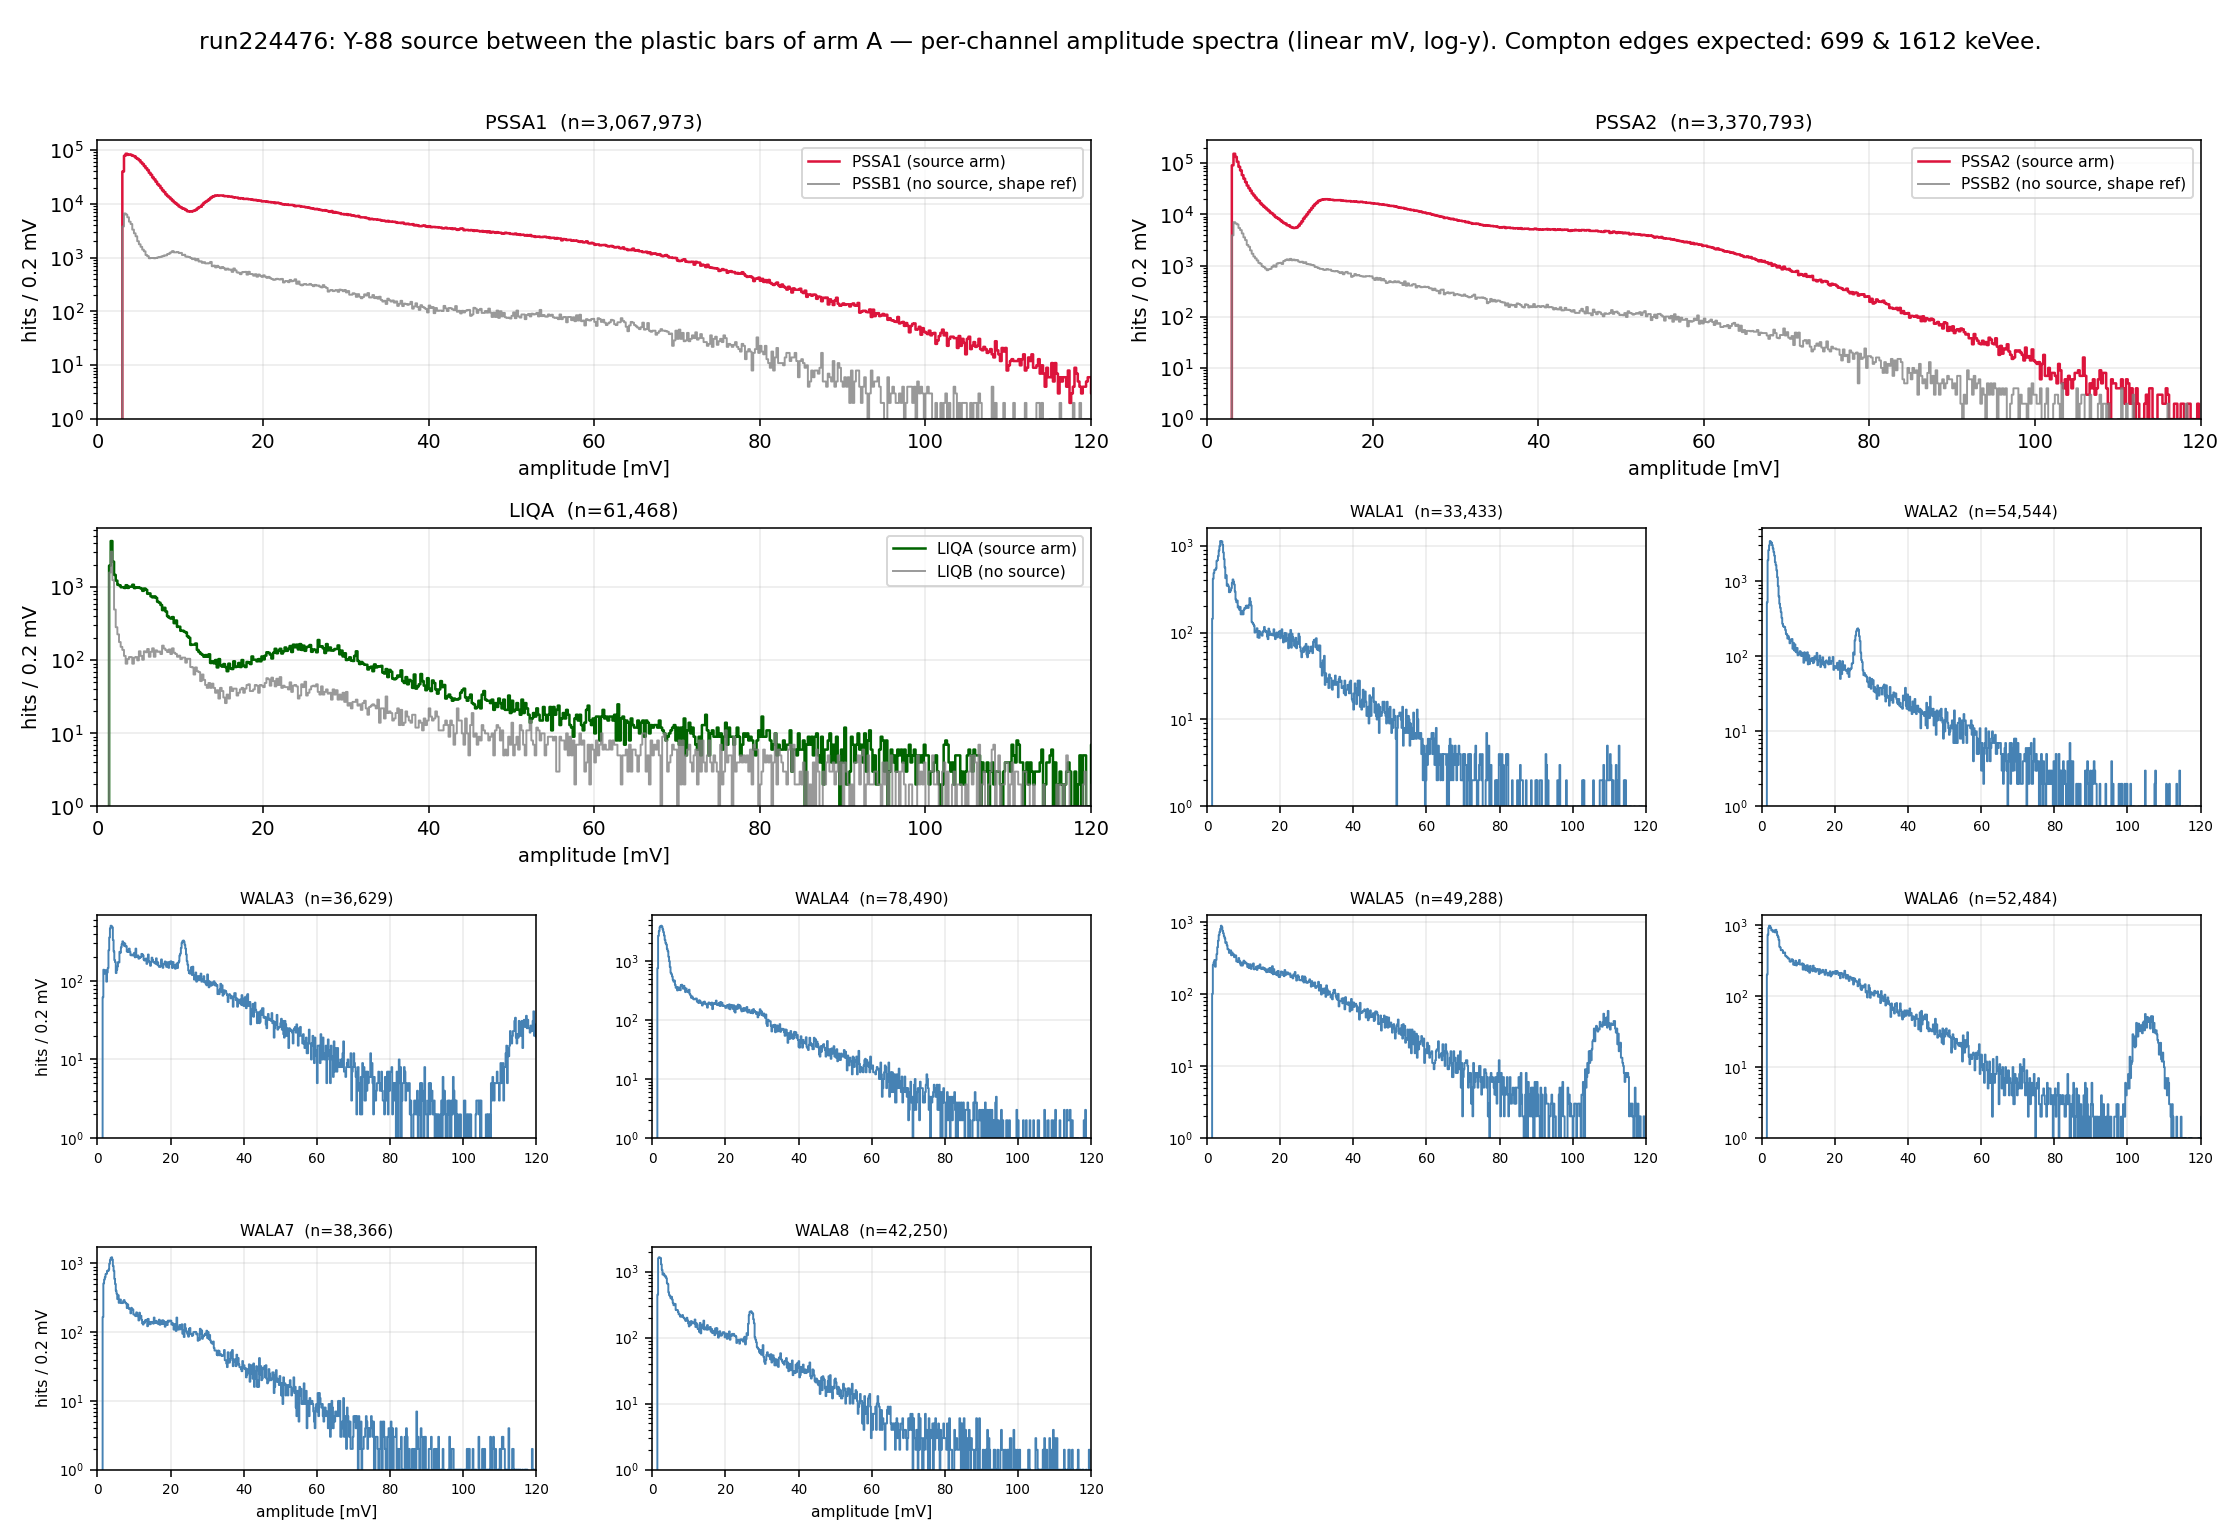
\includegraphics[width=\textwidth]{21_y88/spectra_run224476.png}
\caption{Run 224476 (arm A), per-channel amplitude spectra. Top: the two arm-A
plastics (red) with a non-illuminated arm overlaid as a shape reference (gray).
Middle-left: the arm-A liquid (green) vs.\ a no-source liquid --- a clear
Compton bump near 26\,mV, the first LIQ Y-88 spectrum. Remaining panels: the
eight arm-A SiPM-wall channels (now noise-suppressed by the new PSA);
source-facing bars show a clean edge bump near 26\,mV.}
\label{fig:spectra}
\end{figure}

\section{Plastic Compton edges and linearity}
Figure~\ref{fig:edges} shows the fits; Table~\ref{tab:pss} collects the results.
The 699\,keVee edge (the dominant step) is the robust landmark at 20--27\,mV
across all eight channels; the weaker 1612\,keVee edge follows at 37--64\,mV.
Their measured ratio (median 2.4, Table~\ref{tab:pss}) reproduces the expected
2.31 without being imposed, directly confirming the two-edge interpretation; the
implied nonlinearity is $\lesssim$10--20\%. The per-channel gains span
24--39\,mV/MeVee, all $\sim$20$\times$ the nominal-HV MIP scale
(0.65--2.05\,mV/MeV), so the plastic HV was raised for these runs; the exact
values are not in \texttt{DAQsettings} and are needed to transport the numbers
to nominal.

\begin{figure}[H]\centering
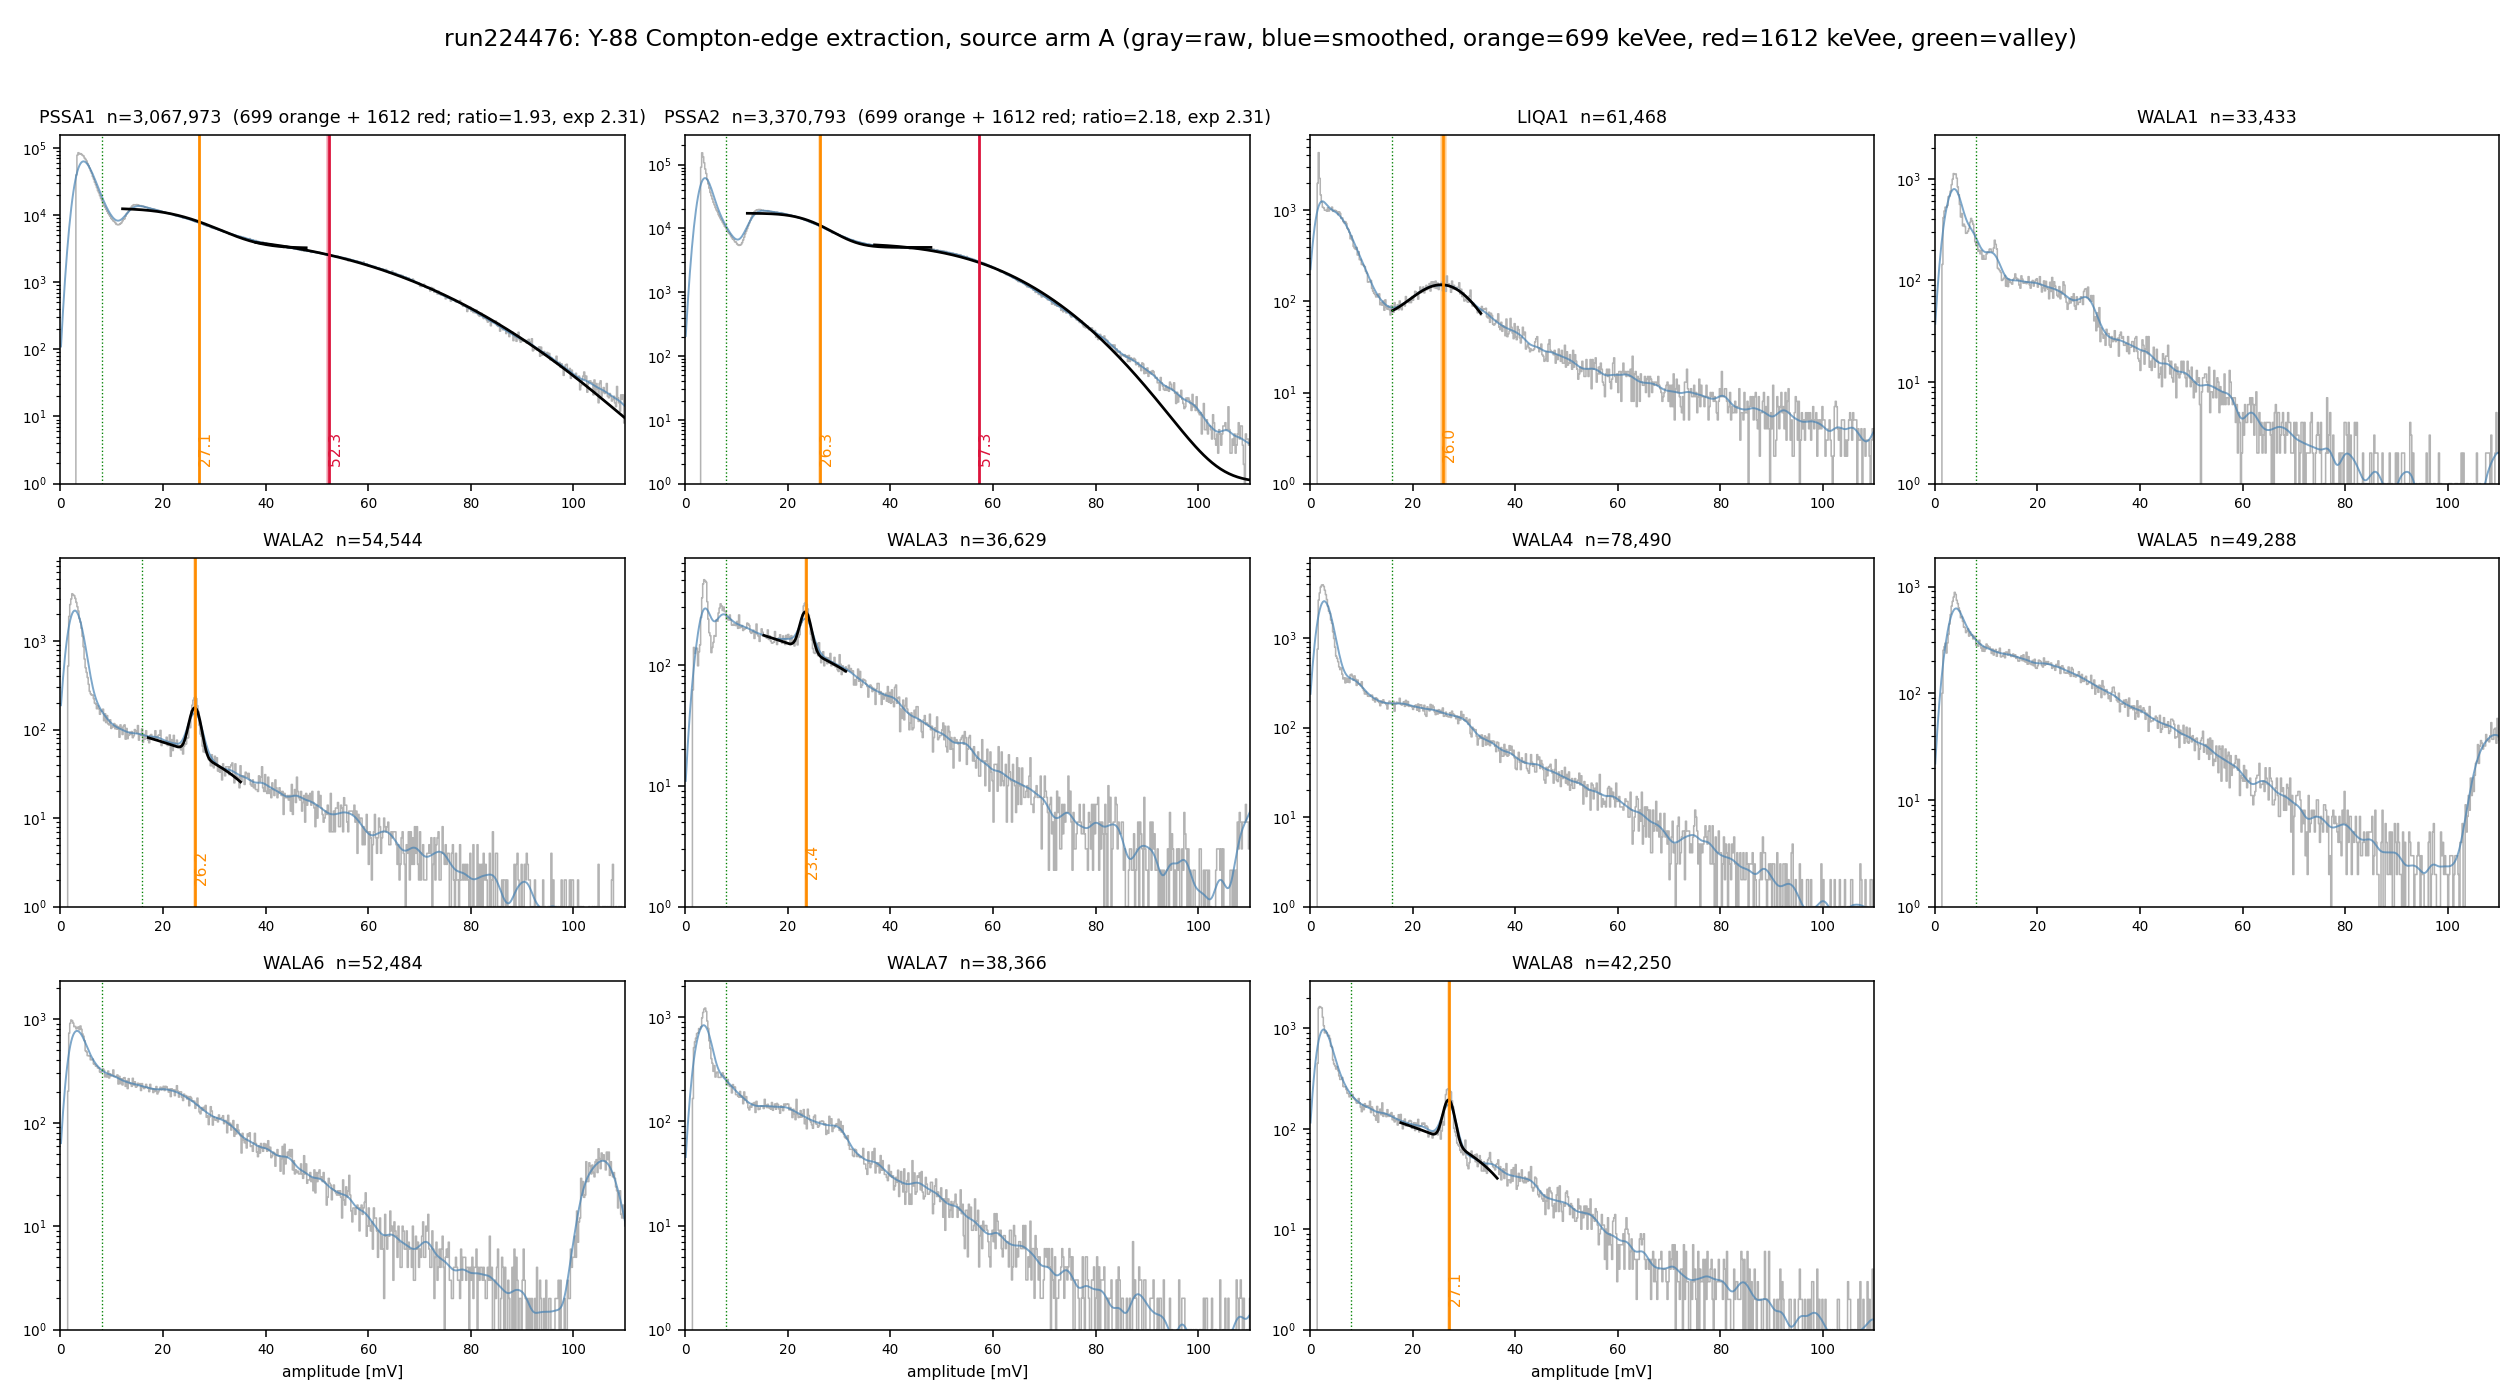
\includegraphics[width=\textwidth]{21_y88/edges_run224476.png}
\caption{Arm-A edge extraction. Gray: raw linear spectrum; blue: smoothed;
black: fitted model; orange/red: the 699/1612\,keVee edges with bootstrap bands;
green dotted: the noise valley. Plastics show the two independent step fits; the
liquid and source-facing walls show the single-bump fit.}
\label{fig:edges}
\end{figure}

\begin{table}[H]\centering
\caption{Plastic Compton edges (mV) at the raised run HV, per channel, from all
four source runs. ``mV/MeVee'' is the through-origin two-point slope; ``ratio''
is the \emph{measured} 1612/699 (expected 2.31); ``nonlin.'' is ratio/2.307.}
\label{tab:pss}
\begin{tabular}{lccccc}
\toprule
channel & 699\,keVee [mV] & 1612\,keVee [mV] & mV/MeVee & ratio & nonlin.\ \\
\midrule
PSSA1 & 27.1 & 52.3 & 33.4 & 1.93 & 0.84 \\
PSSA2 & 26.3 & 57.3 & 35.9 & 2.18 & 0.95 \\
PSSB1 & 20.1 & 50.1 & 30.7 & 2.50 & 1.08 \\
PSSB2 & 23.3 & 59.4 & 36.3 & 2.55 & 1.11 \\
PSSC1 & 22.3 & 55.1 & 33.8 & 2.47 & 1.07 \\
PSSC2 & 19.9 & 46.5 & 28.8 & 2.34 & 1.01 \\
PSSD1 & 24.4 & 63.8 & 38.9 & 2.61 & 1.13 \\
PSSD2 & 20.4 & 36.9 & 23.9 & 1.81 & 0.78 \\
\midrule
median & 22.8 & 54.6 & 33.6 & 2.40 & 1.04 \\
\bottomrule
\end{tabular}
\end{table}

\section{Liquid and SiPM-wall edges}
On the liquids and walls the 699\,keVee edge is a single bump
(Table~\ref{tab:liqwal}). The \textbf{liquid scale is new}: 22--26\,mV
(32--37\,mV/MeVee) on all four vessels, consistent to $\sim$10\% arm-to-arm
despite modest statistics (6--110\,k hits). The walls give 20--30\,mV on the
two-to-three source-facing channels per arm; a couple of channels (e.g.\ WALD7)
scatter high, and channels 5/6 on each arm carry an unrelated narrow peak near
90--105\,mV (an instrumental feature, not the Compton edge) that the fit
ignores. Figure~\ref{fig:calib} (right) compares the 699\,keVee edge across the
three detector types per arm: they view the same source and, although they are
different detectors at independently-set HV, all land within 21--27\,mV.

The run-224404 wall-MIP cross-check from the earlier official-file pass is
\emph{not} repeated here: 224404 was reconstructed with the old PSA while these
runs now use the pulse-shape-fitting PSA, so that comparison is no longer
apples-to-apples. A same-PSA wall MIP (run 224489 was processed with the same
UserInput) would restore it.

\begin{table}[H]\centering
\caption{Liquid and SiPM-wall 699\,keVee Compton-edge bump (mV), source-facing
channels. LIQ is the first absolute LIQ energy scale.}
\label{tab:liqwal}
\begin{tabular}{lcc@{\hskip 2cm}lcc}
\toprule
LIQ & 699 [mV] & mV/MeVee & WAL & 699 [mV] & mV/MeVee \\
\midrule
LIQA & 26.0 & 37.2 & WALA2 & 26.2 & 37.5 \\
LIQB & 22.6 & 32.4 & WALA3 & 23.4 & 33.6 \\
LIQC & 24.0 & 34.4 & WALA8 & 27.1 & 38.7 \\
LIQD & 22.1 & 31.7 & WALB4 & 26.6 & 38.0 \\
      &      &      & WALB5 & 27.0 & 38.6 \\
      &      &      & WALC2 & 21.6 & 30.9 \\
      &      &      & WALC3 & 28.7 & 41.1 \\
      &      &      & WALC8 & 24.1 & 34.5 \\
      &      &      & WALD2 & 26.5 & 37.9 \\
      &      &      & WALD8 & 19.8 & 28.3 \\
\bottomrule
\end{tabular}
\end{table}

\begin{figure}[H]\centering
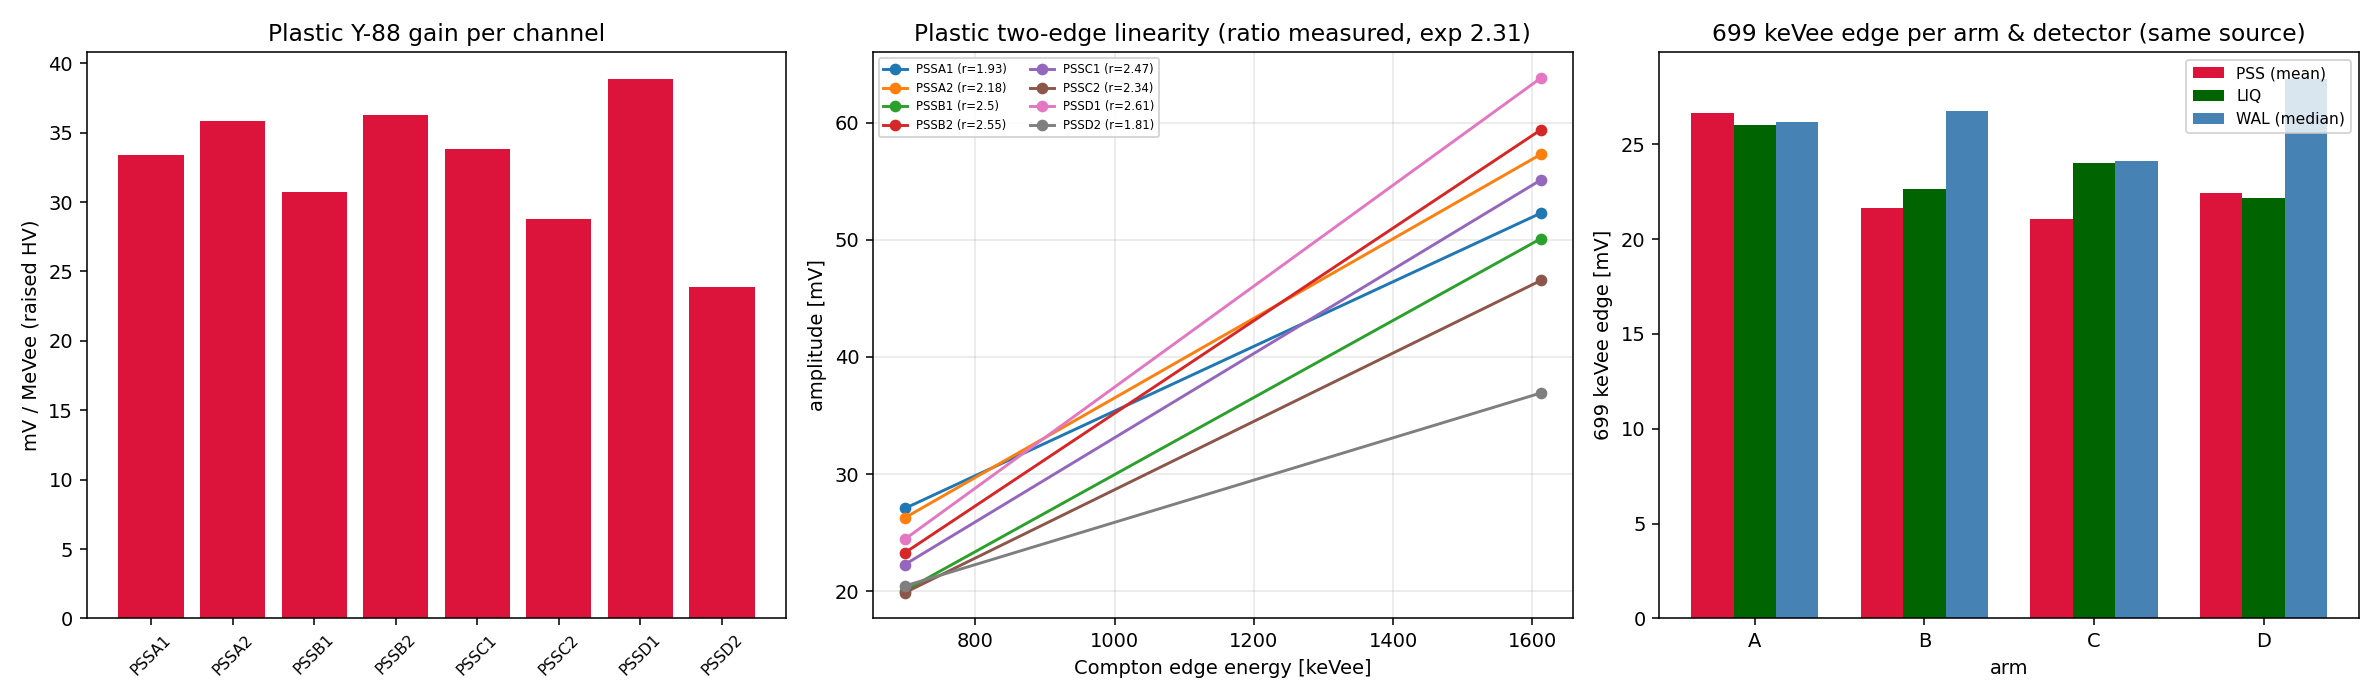
\includegraphics[width=\textwidth]{21_y88/energy_calib.png}
\caption{Left: plastic Y-88 gain per channel (mV/MeVee, raised HV). Middle:
plastic two-edge linearity --- the two Compton edges plus the origin, with the
measured 1612/699 ratio per channel. Right: the 699\,keVee edge per arm for the
three detector types (same source).}
\label{fig:calib}
\end{figure}

\section{Status and open items}
The spectra, per-channel Compton edges (\texttt{calib/y88\_edges\_*.json}) and
the mV/keVee calibration (\texttt{calib/y88\_energy\_calib.json}) are complete
for plastics, liquids, and walls on the reprocessed files. Two items remain:
\begin{enumerate}
\item \textbf{Plastic (and wall) HV during runs 224476--79} --- not in
      \texttt{DAQsettings}; required to transport the plastic edges to nominal
      HV and compare directly with the run-224489 MIP scale.
\item \textbf{Wall MIP cross-check at the same PSA} --- extract the wall MIP from
      run 224489 (same UserInput) to cross-check the Y-88 wall edge without the
      reconstruction mismatch that retired the 224404 comparison.
\end{enumerate}

\end{document}
